% Options for packages loaded elsewhere
\PassOptionsToPackage{unicode}{hyperref}
\PassOptionsToPackage{hyphens}{url}
\PassOptionsToPackage{dvipsnames,svgnames*,x11names*}{xcolor}
%
\documentclass[
]{article}
\usepackage{lmodern}
\usepackage{amssymb,amsmath}
\usepackage{ifxetex,ifluatex}
\ifnum 0\ifxetex 1\fi\ifluatex 1\fi=0 % if pdftex
  \usepackage[T1]{fontenc}
  \usepackage[utf8]{inputenc}
  \usepackage{textcomp} % provide euro and other symbols
\else % if luatex or xetex
  \usepackage{unicode-math}
  \defaultfontfeatures{Scale=MatchLowercase}
  \defaultfontfeatures[\rmfamily]{Ligatures=TeX,Scale=1}
\fi
% Use upquote if available, for straight quotes in verbatim environments
\IfFileExists{upquote.sty}{\usepackage{upquote}}{}
\IfFileExists{microtype.sty}{% use microtype if available
  \usepackage[]{microtype}
  \UseMicrotypeSet[protrusion]{basicmath} % disable protrusion for tt fonts
}{}
\makeatletter
\@ifundefined{KOMAClassName}{% if non-KOMA class
  \IfFileExists{parskip.sty}{%
    \usepackage{parskip}
  }{% else
    \setlength{\parindent}{0pt}
    \setlength{\parskip}{6pt plus 2pt minus 1pt}}
}{% if KOMA class
  \KOMAoptions{parskip=half}}
\makeatother
\usepackage{xcolor}
\IfFileExists{xurl.sty}{\usepackage{xurl}}{} % add URL line breaks if available
\IfFileExists{bookmark.sty}{\usepackage{bookmark}}{\usepackage{hyperref}}
\hypersetup{
  colorlinks=true,
  linkcolor=blue,
  filecolor=Maroon,
  citecolor=Blue,
  urlcolor=Blue,
  pdfcreator={LaTeX via pandoc}}
\urlstyle{same} % disable monospaced font for URLs
\usepackage{graphicx}
\makeatletter
\def\maxwidth{\ifdim\Gin@nat@width>\linewidth\linewidth\else\Gin@nat@width\fi}
\def\maxheight{\ifdim\Gin@nat@height>\textheight\textheight\else\Gin@nat@height\fi}
\makeatother
% Scale images if necessary, so that they will not overflow the page
% margins by default, and it is still possible to overwrite the defaults
% using explicit options in \includegraphics[width, height, ...]{}
\setkeys{Gin}{width=\maxwidth,height=\maxheight,keepaspectratio}
% Set default figure placement to htbp
\makeatletter
\def\fps@figure{htbp}
\makeatother
\setlength{\emergencystretch}{3em} % prevent overfull lines
\providecommand{\tightlist}{%
  \setlength{\itemsep}{0pt}\setlength{\parskip}{0pt}}
\setcounter{secnumdepth}{5}

%% pandoc-secnos: required package
\usepackage{cleveref}

%% pandoc-eqnos: disable brackets around cleveref numbers
\creflabelformat{equation}{#2#1#3}
\newlength{\cslhangindent}
\setlength{\cslhangindent}{1.5em}
\newenvironment{cslreferences}%
  {}%
  {\par}

\author{}
\date{}

\begin{document}

\hypertarget{support-vector-machines}{%
\section{Support Vector Machines}\label{support-vector-machines}}

\hypertarget{introduction}{%
\subsection{Introduction}\label{introduction}}

Suppose that we are given a collection of data made up of samples from
two different classes, and we would like to develop an algorithm that
can distinguish between the two classes. For example, given a picture
that is either a dog or a cat, we'd like to be able to say which of the
pictures are dogs, and which are cats. For another example, we might
want to be able to distinguish ``real'' emails from ``spam.'' This type
of problem is called a \emph{classification} problem.

Typically, one approaches a classification problem by beginning with a
large set of data for which you know the classes, and you use that data
to \emph{train} an algorithm to correctly distinguish the classes for
the test cases where you already know the answer. For example, you start
with a few thousand pictures labelled ``dog'' and ``cat'' and you build
your algorithm so that it does a good job distinguishing the dogs from
the cats in this initial set of \emph{training data}. Then you apply
your algorithm to pictures that aren't labelled and rely on the
predictions you get, hoping that whatever let your algorithm distinguish
between the particular examples will generalize to allow it to correctly
classify images that aren't pre-labelled.

Because classification is such a central problem, there are many
approaches to it. We will see several of them through the course of
these lectures. We will begin with a particular classification algorithm
called ``Support Vector Machines'' (SVM) that is based on linear
algebra. The SVM algorithm is widely used in practice and has a
beautiful geometric interpretation, so it will serve as a good beginning
for later discussion of more complicated classification algorithms.

Incidentally, I'm not sure why this algorithm is called a ``machine'';
the algorithm was introduced in the paper
{[}\protect\hyperlink{ref-vapnik92}{1}{]} where it is called the
``Optimal Margin Classifier'' and as we shall see that is a much better
name for it.

\hypertarget{a-simple-example}{%
\subsection{A simple example}\label{a-simple-example}}

Let us begin our discussion with a very simple dataset (see
{[}\protect\hyperlink{ref-penguins}{2}{]} and
{[}\protect\hyperlink{ref-penguindata}{3}{]}). This data consists of
various measurements of physical characteristics of 344 penguins of 3
different species: Gentoo, Adelie, and Chinstrap. If we focus our
attention for the moment on the Adelie and Gentoo species, and plot
their body mass against their culmen depth, we obtain the following
scatterplot.

\begin{figure}
\hypertarget{fig:penguins}{%
\centering
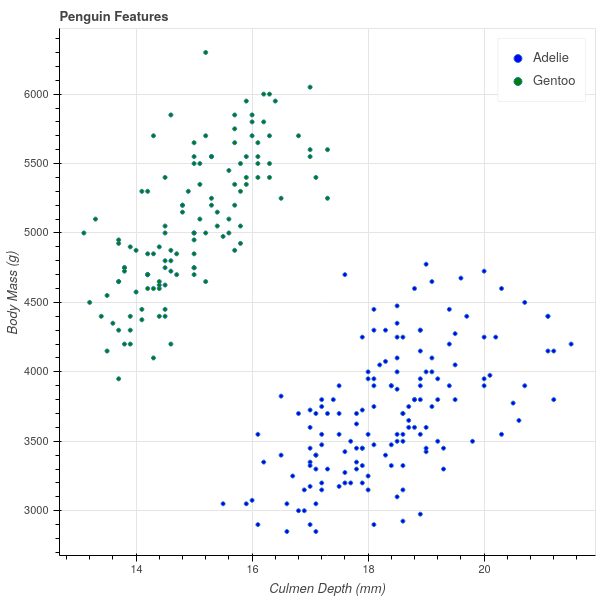
\includegraphics[width=0.5\textwidth,height=\textheight]{../img/penguins.png}
\caption{Penguin Scatterplot}\label{fig:penguins}
}
\end{figure}

Incidentally, a bird's \emph{culmen} is the upper ridge of their beak,
and the \emph{culmen depth} is a measure of the thickness of the beak.
There's a nice picture at {[}\protect\hyperlink{ref-penguindata}{3}{]}
for the penguin enthusiasts.

A striking feature of this scatter plot is that there is a clear
separation between the clusters of Adelie and Gentoo penguins. Adelie
penguins have deeper culmens and less body mass than Gentoo penguins.
These characteristics seem like they should provide a way to classify a
penguin between these two species based on these two measurements.

One way to express the separation between these two clusters is to
observe that one can draw a line on the graph with the property that all
of the Adelie penguins lie on one side of that line and all of the
Gentoo penguins lie on the other. In \cref{fig:penguinsline} I've drawn
in such a line (which I found by eyeballing the picture in
\cref{fig:penguins}). The line has the equation \[
Y = 250X+400.
\]

\begin{figure}
\hypertarget{fig:penguinsline}{%
\centering
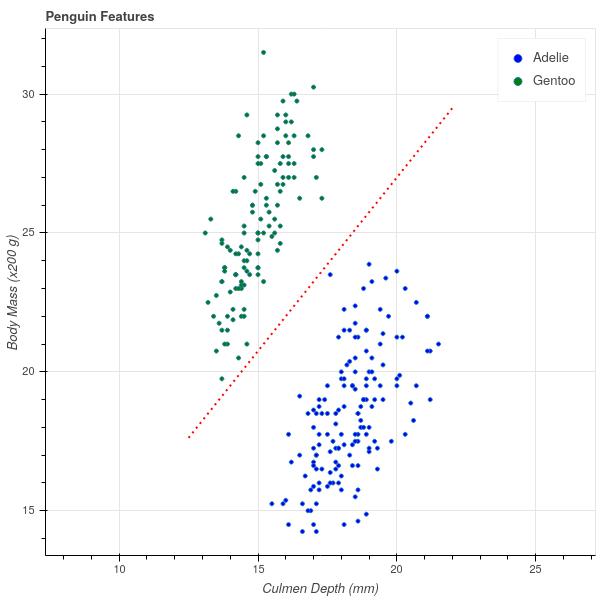
\includegraphics[width=0.5\textwidth,height=\textheight]{../img/penguins_with_line.png}
\caption{Penguins with Separating Line}\label{fig:penguinsline}
}
\end{figure}

The fact that all of the Gentoo penguins lie above this line means that,
for the Gentoo penguins, their body mass in grams is at least \(400\)
more than \(250\) times their culmen depth in mm.

\[
\mathrm{Gentoo\ mass}> 250(\mathrm{Gentoo\ culmen\ depth})+400
\]

while

\[
\mathrm{Adelie\ mass}<250(\mathrm{Adelie\ culmen\ depth})+400.
\]

Now, if we measure a penguin caught in the wild, we can compute
\(250(\mathrm{culmen\ depth})+400\) for that penguin and if this number
is greater than the penguin's mass, we say it's an Adelie; otherwise, a
Gentoo. Based on the experimental data we've collected -- the
\emph{training} data -- this seems likely to work pretty well.

\hypertarget{the-general-case}{%
\subsection{The general case}\label{the-general-case}}

To generalize this approach, let's imagine now that we have \(n\)
samples and \(k\) features (or measurements) for each sample. As before,
we can represent this data as an \(n\times k\) data matrix \(X\). In the
penguin example, our data matrix would be \(344\times 2\), with one row
for each penguin and the columns representing the mass and the culmen
depth. In addition to this numerical data, we have a classification that
assigns each row to one of two classes. Let's represent the classes by a
\(n\times 1\) vector \(Y\), where \(y_{i}=+1\) if the \(i^{th}\) sample
is in one class, and \(y_{i}=-1\) if that \(i^{th}\) sample is in the
other. Our goal is to predict \(Y\) based on \(X\) -- but unlike in
linear regression, \(Y\) takes on the values of \(\pm 1\).

In the penguin case, we were able to find a line that separated the two
classes and then classify points by which side of the line the point was
on. We can generalize this notion to higher dimensions. Before attacking
that generalization, let's recall a few facts about the generalization
to \(\mathbf{R}^{k}\) of the idea of a line.

\hypertarget{hyperplanes}{%
\subsubsection{Hyperplanes}\label{hyperplanes}}

The correct generalization of a line given by an equation
\(w_1 x_1+ w_2 w_2+b=0\) in \(\mathbf{R}^{2}\) is an equation \(f(x)=0\)
where \(f(x)\) is a degree one polynomial \begin{equation}
f(x) = f(x_1,\ldots, x_k) = w_1 x_1 + w_2 x_2 +\cdots + w_k x_k + b 
\label{eq:degreeone}\end{equation}

It's easier to understand the geometry of an equation like \(f(x)=0\) in
\cref{eq:degreeone} if we think of the coefficients \(w_i\) as forming a
\emph{nonzero} vector \(w = (w_1,\ldots, w_k)\) in \(\mathbf{R}^{k}\)
and writing the formula for \(f(x)\) as \[
f(x) = w\cdot x +b
\].

\textbf{Lemma:} Let \(f(x)=w\cdot x+b\) with \(w\in\mathbf{R}^{k}\) a
nonzero vector and \(b\) a constant in \(\mathbf{R}\).

\begin{itemize}
\tightlist
\item
  The inequalities \(f(x)>0\) and \(f(x)<0\) divide up
  \(\mathbf{R}^{k}\) into two disjoint subsets (called half spaces), in
  the way that a line in \(\mathbf{R}^{2}\) divides the plane in half.
\item
  The vector \(w\) is normal vector to the hyperplane \(f(x)=0\).
  Concretely this means that if \(p\) and \(q\) are any two points in
  that hyperplane, then \(w\cdot (p-q)=0\).
\item
  Let \(p=(u_1,\ldots,u_k)\) be a point in \(\mathbf{R}^{k}\). Then the
  perpendicular distance \(D\) from \(p\) to the hyperplane \(f(x)=0\)
  is \[
  D = \frac{f(p)}{\|w\|}
  \]
\end{itemize}

\textbf{Proof:} The first part is clear since the inequalities are
mutually exclusive. For the secon part, suppose that \(p\) and \(q\)
satisfy \(f(x)=0\). Then \(w\cdot p+b = w\cdot q+b=0\). Subtracting
these two equations gives \(w\cdot (p-q)=0\), so \(p-q\) is orthogonal
to \(w\).

For the third part, consider \cref{fig:triangle}. The point \(q\) is an
arbitrary point on the hyperplane defined by the equation
\(w\cdot x+b=0\). The distance from the hyperplane to \(p\) is measured
along the dotted line perpendicular to the hyperplane. The dot product
\(w\cdot (p-q) = \|w\|\|p-q\|\cos(\theta)\) where \(\theta\) is the
angle between \(p-q\) and \(w\) -- which is complementary to the angle
between \(p-q\) and the hyperplane. The distance \(D\) is therefore \[
D=\frac{w\cdot(p-q)}{\|w\|}.
\] However, since \(q\) lies on the hyperplane, we know that
\(w\cdot q+b=0\) so \(w\cdot q = -b\). Therefore
\(w\cdot(p-q)=w\cdot p+b=f(p)\), which is the formula we seek.

\begin{figure}
\hypertarget{fig:triangle}{%
\centering
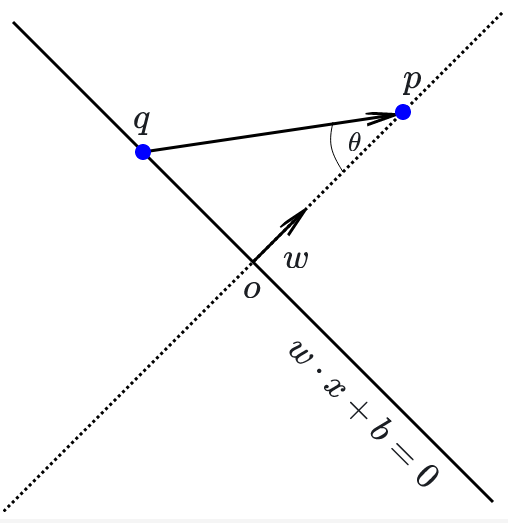
\includegraphics[width=0.3\textwidth,height=\textheight]{../img/triangle.png}
\caption{Distance to a Hyperplane}\label{fig:triangle}
}
\end{figure}

\hypertarget{sec:linearseparable}{%
\subsubsection{Linear separability and
Margins}\label{sec:linearseparable}}

Now we can return to our classification scheme. The following definition
generalizes our two dimensional picture from the penguin data.

\textbf{Definition:} Suppose that we have an \(n\times k\) data matrix
\(X\) and a set of labels \(Y\) that assign the \(n\) samples to one of
two classes. Then the labelled data is said to be \emph{linearly
separable} if there is a vector \(w\) and a constant \(b\) so that, if
\(f(x)=w\cdot x+b\), then \(f(x)>0\) whenever \(x=(x_1,\ldots, x_k)\) is
a row of \(X\) -- a sample -- belonging to the \(+1\) class, and
\(f(x)<0\) whenever \(x\) belongs to the \(-1\) class. The solutions to
the equation \(f(x)=0\) in this situation form a hyperplane that is
called a \emph{separating hyperplane} for the data.

In the situation where our data falls into two classes that are linearly
separable, our classification strategy is to find a separating
hyperplane \(f\) for our training data. Then, given a point \(x\) whose
class we don't know, we can evaluate \(f(x)\) and assign \(x\) to a
class depending on whether \(f(x)>0\) or \(f(x)<0\).

This definition begs two questions about a particular dataset:

\begin{enumerate}
\def\labelenumi{\arabic{enumi}.}
\tightlist
\item
  How do we tell if the two classes are linearly separable?
\item
  If the two sets are linearly separable, there are infinitely many
  separating hyperplanes. To see this, look back at the penguin example
  and notice that we can `wiggle' the red line a little bit and it will
  still separate the two sets. Which is the `best' separating
  hyperplane?
\end{enumerate}

Let's try to make the first of these two questions concrete. We have two
sets of points \(A\) and \(B\) in \(\mathbf{R}^{k}\), and we want to
(try to) find a vector \(w\) and a constant \(b\) so that
\(f(x)=w\cdot x+b\) takes strictly positive values for \(x\in A\) and
strictly negative ones for \(x\in B\). Let's approach the problem by
first choosing \(w\) and then asking whether there is a \(b\) that will
work. In the two dimensional case, this is equivalent to choosing the
slope of our line, and then asking if we can find an intercept so that
the line passes between the two classes.

In algebraic terms, we are trying to solve the following system of
inequalities: given \(w\), find \(b\) so that: \[
w\cdot x+b>0 \hbox{ for all $x$ in A}
\] and \[
w\cdot x+b<0\hbox{ for all $x$ in B}.
\] This is only going to be possible if there is a gap between the
smallest value of \(w\cdot x\) for \(x\in A\) and the largest value of
\(w\cdot x\) for \(x\in B\). In other words, given \(w\) there is a
\(b\) so that \(f(x)=w\cdot x+b\) separates \(A\) and \(B\) if \[
\max_{x\in B}w\cdot x < \min_{x\in A} w\cdot x.
\] If this holds, then choose \(b\) so that \(-b\) lies in this open
interval and you will obtain a separating hyperplane.

\textbf{Proposition:} The sets \(A\) and \(B\) are linearly separable if
there is a \(w\) so that \[
\max_{x\in B}w\cdot x < \min_{x\in A} w\cdot x
\] If this inequality holds for some \(w\), and \(-b\) within this open
interval, then \(f(x)=w\cdot x+b\) is a separating hyperplane for \(A\)
and \(B\).

\Cref{fig:penguinhwy2} is an illustration of this argument for a subset
of the penguin data. Here, we have fixed \(w=(250,-1)\) coming from the
line \(y=250x+400\) that we eyeballed earlier. For each Gentoo (green)
point \(x_{i}\), we computed \(-b=w\cdot x_{i}\) and drew the line
\(f(x) = w\cdot x - w\cdot x_{i}\) giving a family of parallel lines
through each of the green points. Similarly for each Adelie (blue) point
we drew the corresponding line. The maximum value of \(w\cdot x\) for
the blue points turned out to be \(-75\) and the minimum value of
\(w\cdot x\) for the green points turned out to be \(525\). Thus we have
two lines with a gap between them, and any parallel line in that gap
will separate the two sets.

Finally, among all the lines \emph{with this particular \(w\)}, it seems
that the \textbf{best} separating line is the one running right down the
middle of the gap between the boundary lines. Any other line in the gap
will be closer to either the blue or green set that the midpoint line
is.

\begin{figure}
\hypertarget{fig:penguinhwy2}{%
\centering
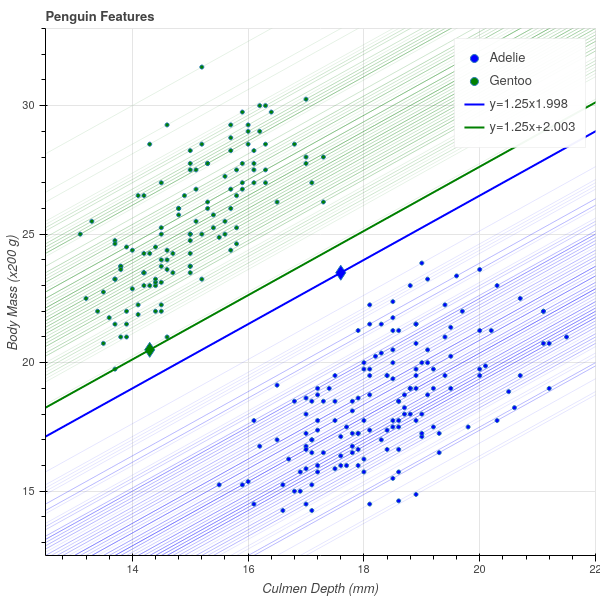
\includegraphics[width=0.5\textwidth,height=\textheight]{../img/penguinhwy2.png}
\caption{Lines in Penguin Data for
\(w=(250,-1)\)}\label{fig:penguinhwy2}
}
\end{figure}

Let's put all of this together and see if we can make sense of it in
general.

Suppose that \(A^{+}\) and \(A^{-}\) are finite point sets in
\(\mathbf{R}^{k}\) and \(w\in\mathbf{R}^{k}\) such that \[
B^{-}(w)=\max_{x\in A^{-}}w\cdot x < \min_{x\in A^{+}}w\cdot x=B^{+}(w).
\] Let \(x^{-}\) be a point in \(A^{-}\) with \(w\cdot x^{-}=B^{-}(w)\)
and \(x^{+}\) be a point in \(A\) with \(w\cdot x^{+}=B^{+}(w)\). The
two hyperplanes \(f^{\pm}(x) = w\cdot x - B^{\pm}\) have the property
that: \[
f^{+}(x)\ge 0\hbox{ for }x\in A^{+}\hbox{ and }f^{+}(x)<0\hbox{ for }x\in A^{-}
\] and \[
f^{-}(x)\le 0\hbox{ for }x\in A^{-}\hbox{ and }f^{-}(x)>0\hbox{ for }x\in A^{+}
\]

Hyperplanes like \(f^{+}\) and \(f^{-}\), which ``just touch'' a set of
points, are called supporting hyperplanes.

\textbf{Definition:} Let \(A\) be a set of points in \(\mathbf{R}^{k}\).
A hyperplane \(f(x)=w\cdot x+b=0\) is called a \emph{supporting
hyperplane} for \(A\) if \(f(x)\ge 0\) for all \(x\in A\) and \(f(x)=0\)
for at least one point in \(A\), or if \(f(x)\le 0\) for all \(x\in A\)
and \(f(x)=0\) for at least one point in \(A\).

The gap between the two supporting hyperplanes \(f^{+}\) and \(f^{-}\)
is called the \emph{margin} between \(A\) and \(B\) for \(w\).

\textbf{Definition:} Let \(f^{+}\) and \(f^{-}\) be as in the discussion
above for point sets \(A^{+}\) and \(A^{-}\) and vector \(w\). Then the
orthogonal distance between the two hyperplanes \(f^{+}\) and \(f^{-}\)
is called the geometric margin \(\tau_{w}(A^{+},A^{-})\) (along \(w\))
between \(A^{+}\) and \(A^{-}\). We have \[
\tau_{w}(A^{+},A^{-})=\frac{B^{+}(w)-B^{-}(w)}{\|w\|}.
\]

Now we can propose an answer to our second question about the best
classifying hyperplane.

\textbf{Definition:} The \emph{optimal margin} \(\tau(A^{+},A^{-})\)
between \(A^{+}\) and \(A^{-}\) is the largest value of \(\tau_{w}\)
over all possible \(w\) for which \(B^{-}(w)<B^{+}(w)\): \[
\tau(A^{+},A^{-}) = \max_{w} \tau_{w}(A^{+},A^{-}).
\] If \(w\) is such that \(\tau_{w}=\tau\), then the hyperplane
\(f(x)=w\cdot x - \frac{(B^{+}+B^{-})}{2}\) is the \emph{optimal margin
classifying hyperplane}.

The optimal classifying hyperplane runs ``down the middle'' of the gap
between the two supporting hyperplanes \(f^{+}\) and \(f^{-}\) that give
the sides of the optimal margin.

We can make one more observation about the maximal margin. If we find a
vector \(w\) so that \(f^{+}(x) = w\cdot x -B^{+}\) and
\(f^{-}(x) = w\cdot x-B^{-}\) are the two supporting hyperplanes such
that the gap between them is the optimal margin, then this gap gives us
an estimate on how close together the points in \(A^{+}\) and \(A^{-}\)
can be. This is visible in \cref{fig:penguinhwy2}, where it's clear that
to get from a blue point to a green one, you have to cross the gap
between the two supporting hyperplanes.

\textbf{Proposition:} The closest distance between points in \(A^{+}\)
and \(A^{-}\) is greater than or equal to the optimal margin: \[
\min_{p\in A^{+},q\in A^{-}} \|p-q\|\ge \tau(A^{+},A^{-})
\].

\textbf{Proof:} We have \(f^{+}(p) = w\cdot p - B^{+}\ge 0\) and
\(f^{-}(q) = w\cdot q -B^{-}\le 0\). These two inequalities imply that
\[
w\cdot (p-q)\ge B^{+}-B^{-}>0.
\] Therefore \[
\|p-q\|\|w\|\ge |w\cdot (p-q)|\ge |B^{+}-B^{-}|
\] and so \[
\|p-q\| \ge \frac{B^{+}-B^{-}}{\|w\|} = \tau(A^{+},A^{-})
\]

If this inequality were always \emph{strict} -- that is, if the optimal
margin equalled the minimum distance between points in the two clusters
-- then this would give us an approach to finding this optimal margin.

Unfortunately, that isn't the case. In \cref{fig:nonstrict}, we show a
very simple case involving only six points in total in which the
distance between the closest points in \(A^{+}\) and \(A^{-}\) is larger
than the optimal margin.

\begin{figure}
\hypertarget{fig:nonstrict}{%
\centering
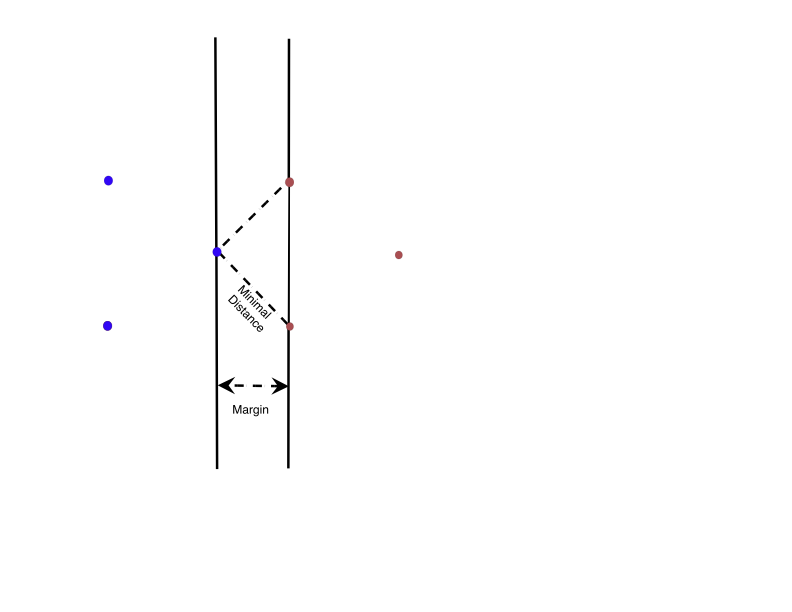
\includegraphics[width=\textwidth,height=3in]{../img/margindistance2.png}
\caption{Shortest distance between + and - points can be greater than
the optimal margin}\label{fig:nonstrict}
}
\end{figure}

At least now our problem is clear. Given our two point sets \(A^{+}\)
and \(A^{-}\), find \(w\) so that \(\tau_{w}(A^{+},A^{-})\) is maximal
among all \(w\) where \(B^{-}(w)<B^{+}(w)\). This is an optimization
problem, but unlike the optimization problems that arose in our
discussions of linear regression and principal component analysis, it
does not have a closed form solution. We will need to find an algorithm
to determine \(w\) by successive approximations. Developing that
algorithm will require thinking about a new concept known as
\emph{convexity.}

\hypertarget{convexity-convex-hulls-and-margins}{%
\subsection{Convexity, Convex Hulls, and
Margins}\label{convexity-convex-hulls-and-margins}}

In this section we introduce the notion of a \emph{convex set} and the
particular case of the \emph{convex hull} of a finite set of points. As
we will see, these ideas will give us a different interpretation of the
margin between two sets and will eventually lead to an algorithm for
finding the optimal margin classifier.

\textbf{Definition:} A subset \(U\) of \(\mathbf{R}^{k}\) is
\emph{convex} if, for any pair of points \(p\) and \(q\) in \(U\), every
point \(t\) on the line segment joining \(p\) and \(q\) also belongs to
\(U\). In vector form, for every \(0\le s\le 1\), the point
\(t(s) = (1-s)p+sq\) belongs to \(U\). (Note that \(t(0)=p\),
\(t(1)=q\), and so \(t(s)\) traces out the segment joining \(p\) to
\(q\).)

\Cref{fig:convexnotconvex} illustrates the difference between convex
sets and non-convex ones.

\begin{figure}
\hypertarget{fig:convexnotconvex}{%
\centering
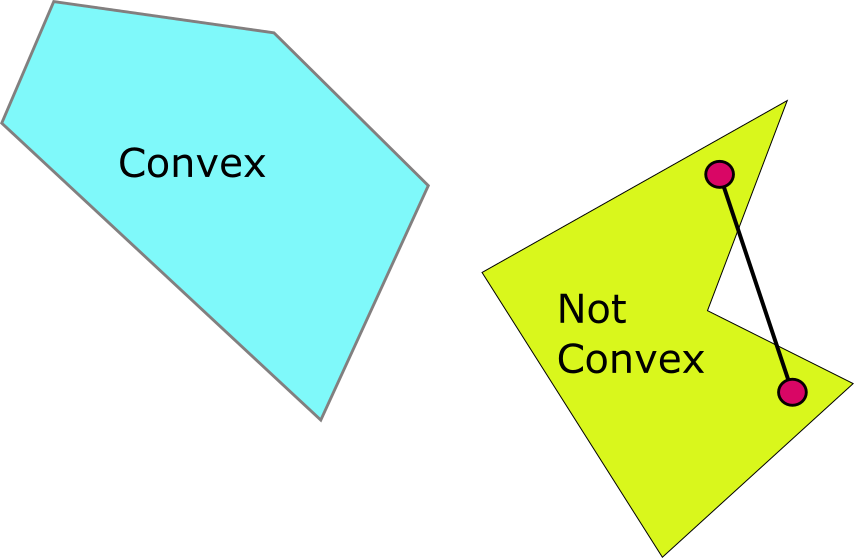
\includegraphics[width=\textwidth,height=3in]{../img/ConvexNotConvex.png}
\caption{Convex vs Non-Convex Sets}\label{fig:convexnotconvex}
}
\end{figure}

The key idea from convexity that we will need to solve our optimization
problem and find the optimal margin is the idea of the \emph{convex
hull} of a finite set of points in \(\mathbf{R}^{k}\).

\textbf{Definition:} Let \(S=\{q_1,\ldots, q_{N}\}\) be a finite set of
\(N\) points in \(\mathbf{R}^{k}\). The \emph{convex hull} \(C(S)\) of
\(S\) is the set of points \[
p = \sum_{i=1}^{N} \lambda_{i}q_{i}
\] as \(\lambda_{1},\ldots,\lambda_{N}\) runs over all positive real
numbers such that \[
\sum_{i=1}^{N} \lambda_{i} = 1.
\]

There are a variety of ways to think about the convex hull \(C(S)\) of a
set of points \(S\), but perhaps the most useful is that it is the
smallest convex set that contains all of the points of \(S\). That is
the content of the next lemma.

\textbf{Lemma:} \(C(S)\) is convex. Furthermore, let \(U\) be any convex
set containing all of the points of \(S\). Then \(U\) contains \(C(S)\).

\textbf{Proof:} To show that \(C(S)\) is convex, we apply the
definition. Let \(p_1\) and \(p_2\) be two points in \(C(S)\), so that
let \(p_{j}=\sum_{i=1}^{N} \lambda^{(j)}_{i}q_{i}\) where
\(\sum_{i=1}^{N}\lambda^{(j)}_{i} = 1\) for \(j=1,2\). Then a little
algebra shows that \[
(1-s)p_1+sp_{2} = \sum_{i=1}^{N} (s\lambda^{(1)}_{i}+(1-s)\lambda^{(2)}_{i})q_{i}
\] and
\(\sum_{i=1}^{N} (s\lambda^{(1)}_{i}+(1-s)\lambda^{(2)}_{i}) = 1\).
Therefore all of the points \((1-s)p_{1}+sp_{2}\) belong to \(C(S)\),
and therefore \(C(S)\) is convex.

For the second part, we proceed by induction. Let \(U\) be a convex set
containing \(S\). Then by the definition of convexity, \(U\) contains
all sums \(\lambda_{i}q_{i}+\lambda_{j}q_{j}\) where
\(\lambda_i+\lambda_j=1\). Now suppose that \(U\) contains all the sums
\(\sum_{i=1}^{N} \lambda_{i}q_{i}\) where exactly \(m-1\) of the
\(\lambda_{i}\) are non-zero for some \(m<N\).\\
Consider a sum \[
q = \sum_{i=1}^{N}\lambda_{i}q_{i}
\] with exactly \(m\) of the \(\lambda_{i}\not=0\). For simplicity let's
assume that \(\lambda_{i}\not=0\) for \(i=1,\ldots, m\). Now let
\(T=\sum_{i=1}^{m-1}\lambda_{i}\) and set \[
q' = \sum_{i=1}^{m-1}\frac{\lambda_{i}}{T}q_{i}.
\] This point \(q'\) belongs to \(U\) by the inductive hypothesis. Also,
\((1-T)=\lambda_{m}\). Therefore by convexity of \(U\), \[
q = (1-T)q_{m}+Tq'
\] also belongs to \(U\). It follows that all of \(C(S)\) belongs to
\(U\).

In \cref{fig:convexhull} we show our penguin data together with the
convex hull of points corresponding to the two types of penguins. Notice
that the boundary of each convex hull is a finite collection of line
segments that join the ``outermost'' points in the point set.

\begin{figure}
\hypertarget{fig:convexhull}{%
\centering
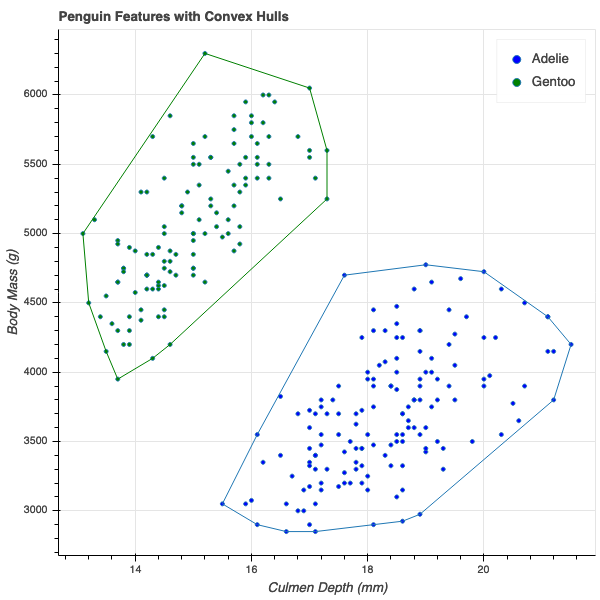
\includegraphics[width=0.5\textwidth,height=\textheight]{../img/penguinswithhulls.png}
\caption{The Convex Hull}\label{fig:convexhull}
}
\end{figure}

One very simple example of a convex set is a half-plane. More
specificically, if \(f(x)=w\cdot x+b=0\) is a hyperplane, then the two
``sides'' of the hyperplane, meaning the subsets \(\{x: f(x)\ge 0\}\)
and \(\{x: f(x)\le 0\}\), are both convex. (This is exercise 1 in
\cref{sec:exercises} ).

As a result of this observation, and the Lemma above, we can conclude
that if \(f(x)=w\cdot x+b=0\) is a supporting hyperplane for the set
\(S\) -- meaning that either \(f(x)\ge 0\) for all \(x\in S\), or
\(f(x)\le 0\) for all \(x\in S\), with at least one point \(x\in S\)
such that \(f(x)=0\) -- then \(f(x)=0\) is a supporting hyperplane for
the entire convex hull. After all, if \(f(x)\ge 0\) for all points
\(x\in S\), then \(S\) is contained in the convex set of points where
\(f(x)\ge 0\), and therefore \(C(S)\) is contained in that set as well.

Interestingly, however, the converse is true as well -- the supporting
hyperplanes of \(C(S)\) are exactly the same as those for \(S\).

\textbf{Lemma:} Let \(S\) be a finite set of points in
\(\mathbf{R}^{k}\) and let \(f(x)=w\cdot +b=0\) be a supporting
hyperplane for \(C(S)\). Then \(f(x)\) is a supporting hyperplane for
\(S\).

\textbf{Proof:} Suppose \(f(x)=0\) is a supporting hyperplane for
\(C(S)\). Let's assume that \(f(x)\ge 0\) for all \(x\in C(S)\) and
\(f(x^{*})=0\) for a point \(x^{*}\in C(S)\), since the case where
\(f(x)\le 0\) is identical. Since \(S\subset C(S)\), we have
\(f(x)\ge 0\) for all \(x\in S\). To show that \(f(x)=0\) is a
supporting hyperplane, we need to know that \(f(x)=0\) for at least one
point \(x\in S\).\\
Let \(x'\) be the point in \(S\) where \(f(x')\) is minimal among all
\(x\in S\). Note that \(f(x')\ge 0\). Then the hyperplane
\(g(x) = f(x)-f(x')\) has the property that \(g(x)\ge 0\) on all of
\(S\), and \(g(x')=0\). Since the halfplane \(g(x)\ge 0\) is convex and
contains all of \(S\), we have \(C(S)\) contained in that halfplane. So,
on the one hand we have \(g(x^{*})=f(x^{*})-f(x')\ge 0\). On the other
hand \(f(x^{*})=0\), so \(-f(x')\ge 0\), so \(f(x')\le 0\). Since
\(f(x')\) is also greater or equal to zero, we have \(f(x')=0\), and so
we have found a point of \(S\) on the hyperplane \(f(x)=0\). Therefore
\(f(x)=0\) is also a supporting hyperplane for \(S\).

This argument can be used to give an alternative description of \(C(S)\)
as the intersection of all halfplanes containing \(S\) arising from
supporting hyperplanes for \(S\). This is exercise 2 in
\cref{sec:exercises}. It also has as a corollary that \(C(S)\) is a
closed set.

\textbf{Lemma:} \(C(S)\) is compact.

\textbf{Proof:} Exercise 2 in \cref{sec:exercises} shows that it is the
intersection of closed sets in \(\mathbf{R}^{k}\), so it is closed.
Exercise 3 shows that \(C(S)\) is bounded. Thus it is compact.

Now let's go back to our optimal margin problem, so that we have
linearly separable sets of points \(A^{+}\) and \(A^{-}\). Recall that
we showed that the optimal margin was at most the minimal distance
between points in \(A^{+}\) and \(A^{-}\), but that there could be a gap
between the minimal distance and the optimal margin -- see
\cref{fig:nonstrict} for a reminder.

It turns out that by considering the minimal distance between
\(C(A^{+})\) and \(C(A^{-})\), we can ``close this gap.'' The following
proposition shows that we can change the problem of finding the optimal
margin into the problem of finding the closest distance between the
convex hulls of \(C(A^{+})\) and \(C(A^{-})\). The following proposition
generalizes the Proposition at the end of \cref{sec:linearseparable}.

\textbf{Proposition:} Let \(A^{+}\) and \(A^{-}\) be linearly separable
sets in \(\mathbf{R}^{k}\). Let \(p\in C(A^{+})\) and \(q\in C(A^{-})\)
be any two points. Then \[
\|p-q\|\ge \tau(A^{+},A^{-}).
\]

\textbf{Proof:} As in the earlier proof, choose supporting hyperplanes
\(f^{+}(x)=w\cdot x-B^{+}=0\) and \(f^{-}(x)=w\cdot x-B^{-}\) for
\(A^{+}\) and \(A^{-}\). By our discussion above, these are also
supporting hyperplanes for \(C(A^{+})\) and \(C(A^{-})\). Therefore if
\(p\in C(A^{+})\) and \(q\in C(A^{-})\), we have \(w\cdot p-B^{+}\ge 0\)
and \(w\cdot q-B^{-}\le 0\). As before \[
w\cdot(p-q)\ge B^{+}-B^{-}>0
\] and so \[
\|p-q\|\ge\frac{B^{+}-B^{-}}{\|w\|\tau_{w}(A^{+},A^{-})}
\] Since this holds for any \(w\), we have the result for
\(\tau(A^{+},A^{-})\).

The reason this result is useful is that, as we've seen, if we restrict
\(p\) and \(q\) to \(A^{+}\) and \(A^{-}\), then there can be a gap
between the minimal distance and the optimal margin. If we allow \(p\)
and \(q\) to range over the convex hulls of these sets, then that gap
disappears.

One other consequence of this is that if \(A^{+}\) and \(A^{-}\) are
linearly separable then their convex hulls are disjoint.

\textbf{Corollary:} If \(A^{+}\) and \(A^{-}\) are linearly separable
then \(\|p-q\|>0\) for all \(p\in C(A^{+})\) and \(q\in C(A^{-})\)

\textbf{Proof:} The sets are linearly separable precisely when
\(\tau>0\).

Our strategy now is to show that if \(p\) and \(q\) are points in
\(C(A^{+})\) and \(C(A^{-})\) respectively that are at minimal distance
\(D\), and if we set \(w=p-q\), then we obtain supporting hyperplanes
with margin equal to \(\|p-q\|\). Since this margin is the \emph{largest
possible margin}, this \(w\) must be the optimal \(w\). This transforms
the problem of finding the optimal margin into the problem of finding
the closest points in the convex hulls.

\textbf{Lemma:} Let \[
D=\min_{p\in C(A^{+}),q\in C(A^{-})} \|p-q\|.
\] Then there are points \(p^*\in C(A^{+})\) and \(q^{*}\in C(A^{-})\)
with \(\|p^{*}-q^{*}\|=D\). If \(p_1^{*},q_1^{*}\) and
\(p_2^{*},q_2^{*}\) are two pairs of points satisfying this condition,
then \(p_1^{*}-q_1^{*}=p_2^{*}-q_{2}^{*}\).

\textbf{Proof:} Consider the set of differences \[
V = \{p-q: p\in C(A^{+}),q\in C(A^{-})\}.
\]

\begin{itemize}
\item
  \(V\) is compact. This is because it is the image of the compact set
  \(C(A^{+})\times C(A^{-})\) in \(\mathbf{R}^{k}\times\mathbf{R}^{k}\)
  under the continuous map \(h(x,y)=x-y\).
\item
  the function \(d(v)=\|v\|\) is continuous and satisfies
  \(d(v)\ge D>0\) for all \(v\in V\).
\end{itemize}

Since \(d\) is a continuous function on a compact set, it attains its
minimum \(D\) and so there is a \(v=p^{*}-q^{*}\) with \(d(v)=D\).

Now suppose that there are two distinct points \(v_1=p_1^*-q_1^*\) and
\(v_2=p_2^*-q_2^*\) with \(d(v_1)=d(v_2)=D\). Consider the line segment
\[
t(s) = (1-s)v_1+sv_2\hbox{ where }0\le s\le 1
\] joining \(v_1\) and \(v_2\).\\
Now \[
t(s) = ((1-s)p_1^*+sp_2^*)-((1-s)q_1^*+sq_2^*).
\] Both terms in this difference belong to \(C(A^{+})\) and \(C(A^{-})\)
respectively, regardless of \(s\), by convexity, and therefore \(t(s)\)
belongs to \(V\) for all \(0\le s\le 1\).

This little argument shows that \(V\) is convex. In geometric terms,
\(v_1\) and \(v_2\) are two points in the set \(V\) equidistant from the
origin and the segment joining them is a chord of a circle; as
\cref{fig:chord} shows, in that situation there must be a point on the
line segment joining them that's closer to the origin than they are.
Since all the points on that segment are in \(V\) by convexity, this
would contradict the assumption that \(v_1\) is the closet point in
\(V\) to the origin.

\begin{figure}
\hypertarget{fig:chord}{%
\centering
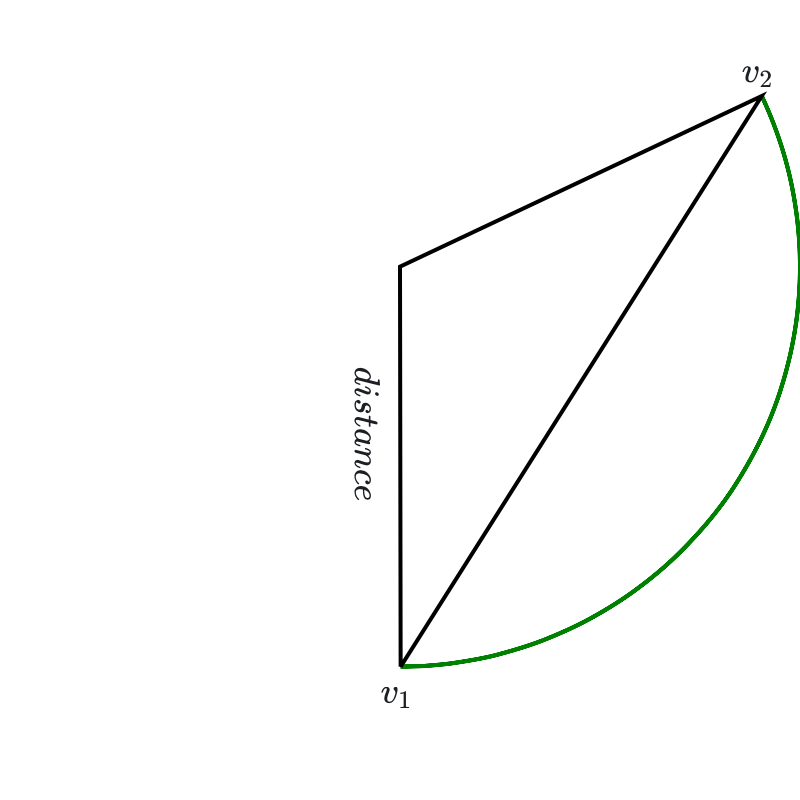
\includegraphics[width=3in,height=\textheight]{../img/chord2.png}
\caption{Chord of a circle}\label{fig:chord}
}
\end{figure}

In algebraic terms, since \(D\) is the minimal value of \(\|v\|\) for
all \(v\in V\), we must have \(t(s)\ge D\).\\
On the other hand \[
\frac{d}{ds}\|t(s)\|^2 = \frac{d}{ds}(t(s)\cdot t(s)) =t(s)\cdot \frac{dt(s)}{ds} = t(s)\cdot(v_2-v_1).
\] Therefore \[
\frac{d}{ds}\|t(s)\|^2|_{s=0} = v_{1}\cdot(v_{2}-v_{1})=v_{1}\cdot v_{2}-\|v_{1}\|^2\le 0
\] since \(v_{1}\cdot v_{2}\le D^{2}\) and \(\|v_{1}\|^2=D^2\). If
\(v_{1}\cdot v_{2}<D^{2}\), then this derivative would be negative,
which by the mean value theorem would mean that there is a value of
\(s\) where \(t(s)\) would be less than \(D\). Since that can't happen,
we conclude that \(v_{1}\cdot v_{2}=D^{2}\) which means that
\(v_{1}=v_{2}\) -- the vectors have the same magnitude \(D\) and are
parallel. This establishes uniqueness.

\textbf{Note:} The essential ideas of this argument show that a compact
convex set in \(\mathbf{R}^{k}\) has a unique point closest to the
origin. The convex set in this instance, \[
V=\{p-q:p\in C(A^{+}),q\in C(A^{-})\},
\] is called the difference \(C(A^{+})-C(A^{-})\), and it is generally
true that the difference of convex sets is convex.

Now we can conclude this line of argument.

\textbf{Theorem:} Let \(p\) and \(q\) be points in \(C(A^{+})\) and
\(C(A^{-})\) respectively are such that \(\|p-q\|\) is minimal among all
such pairs. Let \(w=p-q\) and set \(B^{+}=w\cdot p\) and
\(B^{-}=w\cdot q\). Then \(f^{+}(x)=w\cdot x-B^{+}=0\) and
\(f^{-}(x)=w\cdot x-B^{-}\) are supporting hyperplanes for \(C(A^{+})\)
and \(C(A^{-})\) respectively and the associated margin \[
\tau_{w}(A^{+},A^{-})=\frac{B^{+}-B^{-}}{\|w\|} = \|p-q\|
\] is optimal.

\textbf{Proof:} First we show that \(f^{+}(x)=0\) is a supporting
hyperplane for \(C(A^{+})\). Suppose not. Then there is a point
\(p'\in C(A^{+})\) such that \(f^{+}(x)<0\). Consider the line segment
\(t(s) = (1-s)p+sp'\) running from \(p\) to \(p'\). By convexity it is
entirely contained in \(C(A^{+})\). Now look at the distance from points
on this segment to \(q\): \[
D(s)=\|t(s)-q\|^2.
\] We have \[
\frac{dD(s)}{ds}|_{s=0} = 2(p-q)\cdot (p'-p) = 2w\cdot (p'-p) = 2\left[(f^{+}(p')+B^{+})-(f^{+}(p)+B^{+})\right]
\] so \[
\frac{dD(s)}{ds}|_{s=0} = 2(f^{+}(p')-f^{+}(p))<0
\] since \(f(p)=0\). This means that \(D(s)\) is decreasing along
\(t(s)\) and so by the mean value theorem there is a point \(s'\) along
\(t(s)\) where \(\|t(s')-q\|<D\). This contradicts the fact that \(D\)
is the minimal distance. The same argument shows that \(f^{-}(x)=0\) is
also a supporting hyperplane.

Now the margin for this \(w\) is \[
\tau_{w}(A^{+},A^{-}) = \frac{w\cdot (p-q)}{\|w\|} = \|p-q\|=D
\] and as \(w\) varies we know this is the largest possible \(\tau\)
that can occur. Thus this is the maximal margin.

To recap, we have shown that

\begin{quote}
\textbf{To find \(w\) yielding the maximal margin pair of supporting
hyperplanes, find points \(p\in C(A^{+})\) and \(q\in C(A^{-})\) that
minimize \(\|p-q\|\) and set \(w=p-q\).}
\end{quote}

\Cref{fig:strict} shows how considering the closest point in the convex
hulls ``fixes'' the problem that we saw in \cref{fig:nonstrict}. The
closest point occurs at a point on the boundary of the convex hull that
is not one of the points in \(A^{+}\) or \(A^{-}\).

\begin{figure}
\hypertarget{fig:strict}{%
\centering
\includegraphics[width=0.5\textwidth,height=\textheight]{../img/convexhullwithmargin.png}
\caption{Closest distance between convex hulls gives optimal
margin}\label{fig:strict}
}
\end{figure}

\hypertarget{sec:exercises}{%
\subsection{Exercises}\label{sec:exercises}}

\begin{enumerate}
\def\labelenumi{\arabic{enumi}.}
\item
  Prove that, if \(f(x)=w\cdot x+b=0\) is a hyperplane in
  \(\mathbf{R}^{k}\), then the two ``sides'' of this hyperplane,
  consisting of the points where \(f(x)\ge 0\) and \(f(x)\le 0\), are
  both convex sets.
\item
  Prove that \(C(S)\) is the intersection of all the halfplanes
  \(f(x)\ge 0\) as \(f(x)=w\cdot x+b\) runs through all supporting
  hyperplanes for \(S\) where \(f(x)\ge 0\) for all \(p\in S\).
\item
  Prove that \(C(S)\) is bounded. Hint: show that \(S\) is contained in
  a sphere of sufficiently large radius centered at zero, and then that
  \(C(S)\) is contained in that sphere as well.
\end{enumerate}

\hypertarget{bibliography}{%
\section*{References}\label{bibliography}}
\addcontentsline{toc}{section}{References}

\hypertarget{refs}{}
\begin{cslreferences}
\leavevmode\hypertarget{ref-vapnik92}{}%
{[}1{]} \textsc{Boser}, B., \textsc{Guyon}, I. and \textsc{Vapnik}, V. A
training algorithm for optimal margin classifiers. In \emph{Colt '92:
Proceedings of the fifth annual workshop on computational learning
theory} (D. Haussler, ed) pp 144--52. ACM.

\leavevmode\hypertarget{ref-penguins}{}%
{[}2{]} \textsc{KB}, G., \textsc{TD}, W. and \textsc{WR}, F. (2014).
Ecological sexual dimorphism and environmental variability within a
community of antarctic penguins (genus pygoscelis). \emph{PLoS ONE}
\textbf{9(3)} --13.

\leavevmode\hypertarget{ref-penguindata}{}%
{[}3{]} \textsc{Horst}, A. Palmer penguins.Available at
\url{https://https://github.com/allisonhorst/palmerpenguins}.
\end{cslreferences}

\end{document}
